%%%%%%%%%%%%%%%%%%%%%%%%%%%%%%%%%%%%%%%%%
% Presentation Template
% LaTeX Template
% Version 2.2 (2023-07-17)
%
% This template was adapted by:
% Jonathan Decker (jonathan.decker@uni-goettingen.de)
% From a template made by:
% Julian Kunkel (julian.kunkel@gwdg.de)
%
%%%%%%%%%%%%%%%%%%%%%%%%%%%%%%%%%%%%%%%%%
\documentclass[compress,aspectratio=169]{beamer}

% make sure the theme and config files are on this path
\usepackage[GI]{assets/beamerConfig}

% Used to create mindmaps
\usepackage{tikz}
\usetikzlibrary{mindmap}


\addbibresource{ref.bib}
\graphicspath{{.}{assets/}}

% --- document configuration ---
\newcommand{\mytitle}{Going public}
% Leave empty for no subtitle
\newcommand{\mysubtitle}{Tips for publishing your own code}
\newcommand{\myauthor}{Marc-Philipp Knechtle}
\newcommand{\myauthorurl}{}
\newcommand{\myvenue}{Informatik 2023}
% For example, use \today
\newcommand{\mydate}{\today}
% For example, Institute for Computer Science / GWDG
\newcommand{\myinstitute}{JMU Würzburg}

\configuretitlepage

\begin{document}

	\begin{frame}[plain]
		\titlepage
	\end{frame}

	\begin{frame}[t]{Table of contents}
		\tableofcontents[subsectionstyle=hide/hide]
	\end{frame}

	% --- slides begin ---

	\section{Hide your secrets!}

		\begin{frame}{Sensitive data in git}
			\begin{itemize}
				\item Problem: (Accidental) commits of secrets
				\item e.g. passwords, application secret keys, OAuth secret keys, SSH keys
				\item The file is still accessible in history, even if the original file was deleted
				\item Security risk, even in private repositories
			\end{itemize}	
		% asdf \cite{github2023removing}
		\end{frame}

		\begin{frame}{Removing sensitive data}
			\begin{itemize}
				\item git filter-repo
				\item BFG Repo-Cleaner
			\end{itemize}
		\end{frame}
		
		\begin{frame}{Encrypt sensitive data}
			Methods for encrypting and storing sensitive data:
			\begin{itemize}
				\item 	Why shouldn't I store the secrets separate from the repository?
				\item 	Methods for encrypting and storing sensitive data:
						\begin{itemize}
							\item git-secret CLI 
							\item github encrypted secrets
							\item technology specific encryption tool (e.g. ansible-vault)
						\end{itemize}
			\end{itemize}
		\end{frame}

	
	\section{Creating a healthy community}
		\begin{frame}{Points of interaction with the community}
			\begin{center}
			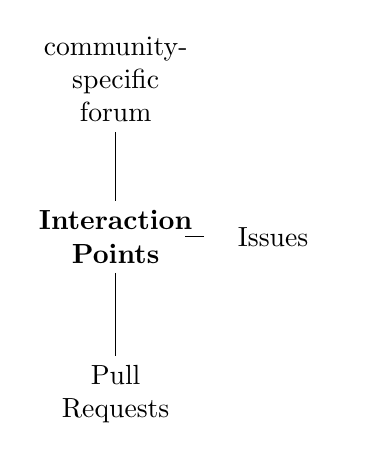
\begin{tikzpicture}[grow cyclic, text width=2cm, align=flush center, level 1/.style={level distance=2cm,sibling angle=90}]
				\node{\textbf{Interaction Points}}
				child{ node {Pull Requests}}
				child{ node {Issues}}
				child{ node {community-specific forum}}		
				;
			\end{tikzpicture}
			\end{center}
		
		\end{frame}
	
		\begin{frame}{Code of Conduct}
			\begin{itemize}
				\item Content: set of rules, with norms, responsibilities and proper parties
				\item defines the actions of a single person in a organisation
				\item Goal: healthy, constructive community behaviour
				\item \texttt{CODE\textunderscore OF\textunderscore CONDUCT} file (in the git repository)
				\item e.g. Contributor Covenant \footnote{https://www.contributor-covenant.org/}, Django Code of Conduct \footnote{\url{https://www.djangoproject.com/conduct/}}
			\end{itemize}				
		\end{frame}
	
	\section{Consistency achieved with continuous integration}	
		\begin{frame}{Continuous Integration overview}
			\begin{figure}
			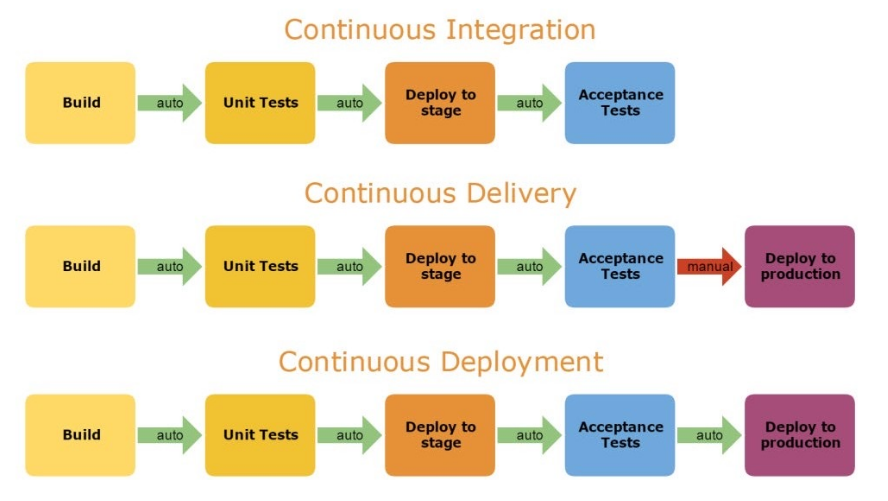
\includegraphics[width=10cm]{assets/ci-overview.png}
			\caption{Comparison CI/CD %\cite{wang2018x}
			}
			\end{figure}
		\end{frame}
		
		\begin{frame}{Github Actions}
			\begin{itemize}
				\item 	CI/CD platform, used for testing Pull Requests
				\item 	Reactions on other events such as an issue beeing created
				\item 	workflows can run on VMs or a self-hosted instance
				\item 	workflows consist of jobs, which is a shell script or an action
				\item 	actions are custom github actions applications (e.g. pulling a repository, setting up the toolchain) 
				\item 	runners are the servers on which the process is performed
			\end{itemize}
		\end{frame}
		
	%\section{Documentation}
	%	\begin{frame}{Documentation}
	%		\begin{itemize}
	%			\item 	Technology specific documentation toolchain (e.g. javadoc)
	%		\end{itemize}
	%	\end{frame}
	
	\section{Promote your code}
	
		\begin{frame}{Ideas for promoting your code}
		
			\begin{itemize}
				\item Cross-promoting projects through their documentation
				\item Writing a blog with shareable posts for each major release
				\item Monitor new mentions of your project e.g. through bots \footnote{\url{https://f5bot.com/}}, help with additional information on these mentions
				
			\end{itemize}
			
		\end{frame}
	
		
		\begin{frame}{References}
			% References slide in appendix
			\renewcommand*{\bibfont}{\normalfont\scriptsize}
			\printbibliography[heading=none]
			\label{pg:lastpage} % Label on the last frame to get the page number on the footer
		\end{frame}

\end{document}
